\documentclass[11pt, a4paper]{article}

\usepackage{amsmath}
\usepackage{amssymb}

% fonts
\usepackage{xeCJK}
\setCJKmainfont[BoldFont=SimHei]{SimSun}
\setCJKfamilyfont{hei}{SimHei}
\setCJKfamilyfont{kai}{KaiTi}
\setCJKfamilyfont{fang}{FangSong}
\newcommand{\hei}{\CJKfamily{hei}}
\newcommand{\kai}{\CJKfamily{kai}}
\newcommand{\fang}{\CJKfamily{fang}}

% style
\usepackage[top=2.54cm, bottom=2.54cm, left=3.18cm, right=3.18cm]{geometry}
\linespread{1.5}
% \usepackage{indentfirst}
\parindent 2em
% \punctstyle{quanjiao}
% \renewcommand{\today}{\number\year 年 \number\month 月 \number\day 日}

% figures and tables
\usepackage{graphicx}
\usepackage[font={bf, footnotesize}, textfont=md]{caption}
\makeatletter
    \newcommand\fcaption{\def\@captype{figure}\caption}
    \newcommand\tcaption{\def\@captype{table}\caption}
\makeatother
\usepackage{booktabs}
\renewcommand\figurename{Figure}
\renewcommand\tablename{Table}
\newcommand{\fref}[1]{\textbf{Figure \ref{#1}}}
\newcommand{\tref}[1]{\textbf{Table \ref{#1}}}
\newcommand{\tabincell}[2]{\begin{tabular}{@{}#1@{}}#2\end{tabular}} % multiply lines in one grid

\usepackage{listings}
\lstset{basicstyle=\ttfamily}

\usepackage{clrscode}
\usepackage{url}

% start of document
\title{\textbf{N-body Report}}
\author{\kai 朱俸民}
\date{\today}

\begin{document}

\maketitle

\section{Introduction}

This project solves the classical N-body problem on both CPU (pthread version) and GPU (cuda version) with XWindow support (to display the locations of bodies).

\section{Barnes-Hut Algorithm}

\subsection{Overview}

In order to solve large scale N-body problem, we use Barnes-Hut algorithm (BHA). The time complexity of the classical brute-force algorithm, say computing force pair by pair, is $O(n^2)$, where $n$ notates the total number of bodies. When the sample size is large, it takes a huge time to solve. However, the time complexity of BHA is $O(n \log n)$. BHA uses a quad-tree (for 2D samples) to organize data. When computing the force, we traverse the tree from the root node but we stop when we either reach the leaf node or the area is far away from the body (we use a threshold to measure), for the latter, we regard all bodies in that area as a signal area (body). Constructing the tree requires a time of $O(n \log n)$, and so does computing all the forces. Thus, BHA is a better way to solve N-body problem.

\subsection{Node Types}

To continue the description of the algorithm, we define the following three types of tree node:

\begin{itemize}
    \item \textit{Empty node}\quad nodes haven't been used yet
    \item \textit{External node}\quad nodes that contains only one body but no children expanded yet
    \item \textit{Internal node}\quad nodes that has children
\end{itemize}

\subsection{Tree Construction}

For each body $b$ to insert at node $x$, follow the recursive method:

\begin{itemize}
    \item if $x$ is an empty node, put $b$ here;
    \item otherwise, update total mass and center of mass for $x$, if $x$ is external node, create its four children and recursively insert the original body of $b$ at proper children nodes;
    \item finally, insert $b$ at proper children nodes of $x$.
\end{itemize}

\subsection{Tree Search}

To calculate the net force acting on each body $b$, use the following recursive procedure, starting with the root of the quad-tree, and let $x$ be the current node:

\begin{itemize}
    \item if $x$ is an external node, calculate the force exerted by the body at $x$ and add this to $b$'s not force;
    \item otherwise, calculate $w / d$, where $w$ notates the length of the current area and $d$ notates the distance between $b$ and $x$. If $w / d < \theta$, where $\theta$ notates the threshold value (given by user), then treat $x$ as a single body whose mass is the total mass of $x$ and position is the center of mass of $x$. Calculate the force exerted by this and add it to $b$'s not force;
    \item otherwise, recursively search at all non-empty children node of $x$.
\end{itemize}

By this method, no empty nodes will be searched.

\section{Parallel Program Implementation}

\subsection{Overview}

We focus parallel methods on computing forces. We use sequential method for tree constructing since the computing part, not the constructing part, is the bottleneck for this problem.

To keep things simple and clear, if we have $n$ bodies, we divide the whole computing problems into exactly $n$ tasks. That is to say, we need to compute the force for each of the $n$ bodies. When we compute on GPU, we simply let each thread do one of these tasks. When we compute on CPU, we divide tasks into equally parts for each thread. Since we are only allowed to use a small number of threads compared with GPU, each threads will do a couple of tasks.

\subsection{Non-recursive Version for Tree Search}

BHA introduce a recursive method of tree search. Actually, we find that the recursive method is the depth first search (DFS) of the tree. Thus, we use a stack to store the nodes indexes and we can simulate the recursive calling of the search function: when we reach external node, we stop here; when we reach internal node, we push its non-empty children into stack. Every time, we pop a node from stack to do the routine described above. Thus, we finish the searching process without recursively calling function. We set the stack size as 64 nodes (integers).

We find that this non-recursive method has the following advantages:

\begin{itemize}
    \item function calling time is saved, and
    \item minimize the stack memory resource, making better performance on GPU.
\end{itemize}

\subsection{Pthread Version}

Suppose that $m$ threads are created, the first $m-1$ threads each compute $\lceil n/m \rceil$ bodies and the last thread compute the remaining $n - m\lceil n/m \rceil$ bodies.

\subsection{Cuda Version}

We use $\lceil n/512 \rceil$ blocks and 512 threads in each block. For those threads who are out of bound, they do nothing.

\subsection{Rebounce Strategy}

With the increase of iteration, bodies are tend to be further and further away from the area center. In order to control the largest area these bodies locale, we use a ``rebounce strategy'' to avoid it. The idea is rather simple, after updating the positions of each body in an iteration, we check whether each body is now out of bound (the area square of the root node, which is the largest). If it is out of bound, we reverse its velocity direction, which simulates a reboucing.

\section{Performance Results for Different Parameters}

\subsection{Tree Constructing}

For the given test cases, we measure the time cost (ms, the same in the following paragraphs) as shown in \tref{treecons}. Note that we compute 10 iterations with mass 1 and time interval 0.5. We show the average time cost, and the maximum tree depth and maximum number of nodes (including empty nodes) we used in the first 10 iterations.

\begin{center}
    \tcaption{Performance on different number of threads}\label{treecons}
    \begin{tabular}{ccccc}
        \toprule
        test case & sample size & time cost & depth & number of nodes \\
        \midrule
        \texttt{test1.txt} & 945 & 1.05 & 8 & 2753 \\
        \texttt{test2.txt} & 81921 & 80.5 & 22 & 236581 \\
        \texttt{test3.txt} & 1923840 & 2936.0 & 23 & 5558209 \\
        \texttt{test4.txt} & 7283942 & 13587.2 & 25 & 21021713 \\
        \bottomrule
    \end{tabular}
\end{center}

\begin{center}
    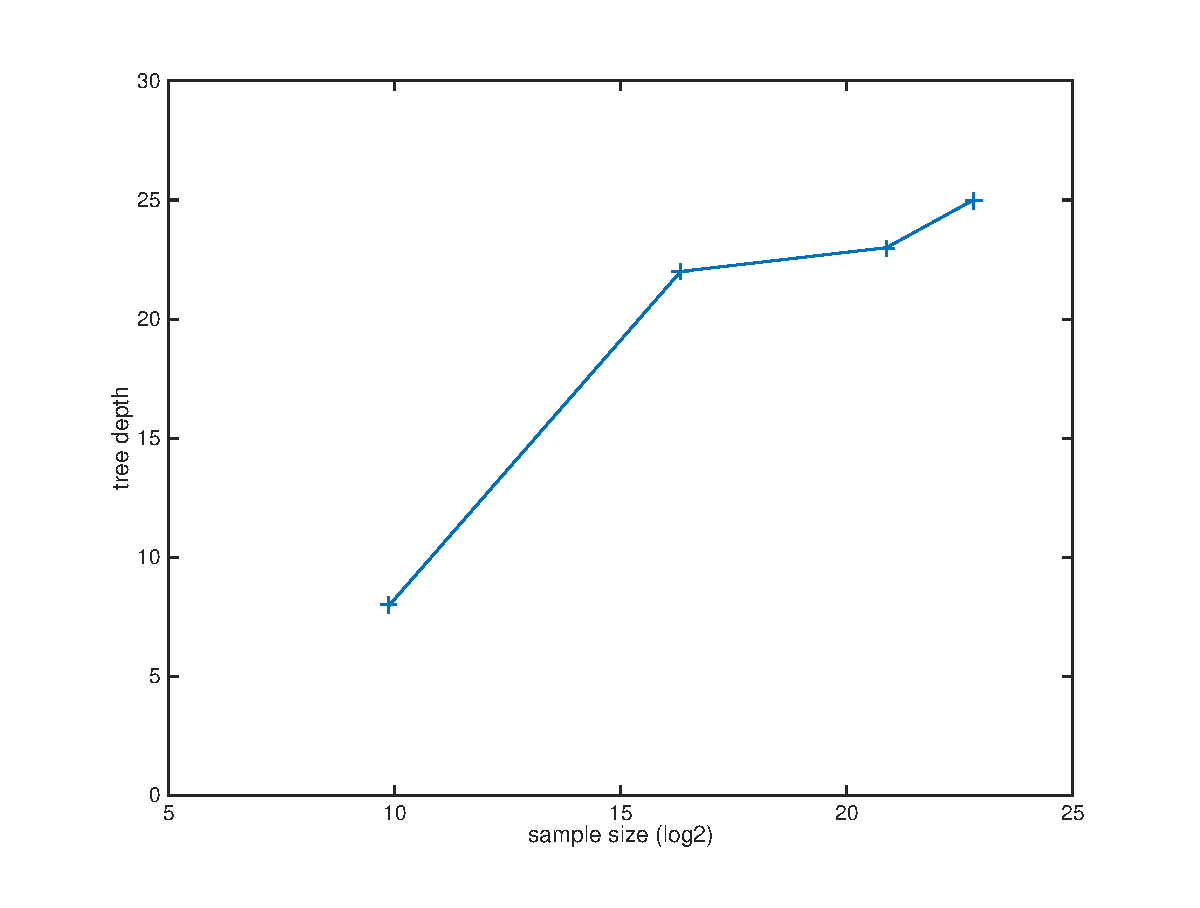
\includegraphics[width=12cm]{depth}
    \fcaption{Tree depth for test cases}
\end{center}

It is interesting to see that the maxinum depth is less than 30 and the number of nodes is less than three times of sample size. By this experiment, it is reasonable and safe for us to set the recursive stack size as 64 and the array length of tree as four times of sample size. Besides, since the tree depth is small, BHA requires much less computational time than brute-force method even if the sample size is rather huge.

\subsection{Stability Among Iterations}

We use \texttt{test1.txt} as test case and we compute 1000 iterations with mass 1, time interval 0.5 and threshold 0. We analyze the time cost for each iteration for both pthread version and cuda version. Results are shown in \fref{time_p} and \fref{time_c} respectively. Please note that the time of computing only contains the force computing part (tree constructing part is excluded) and the time we shown is the average value each iteration costs (the same for the following paragraphs).

\begin{center}
    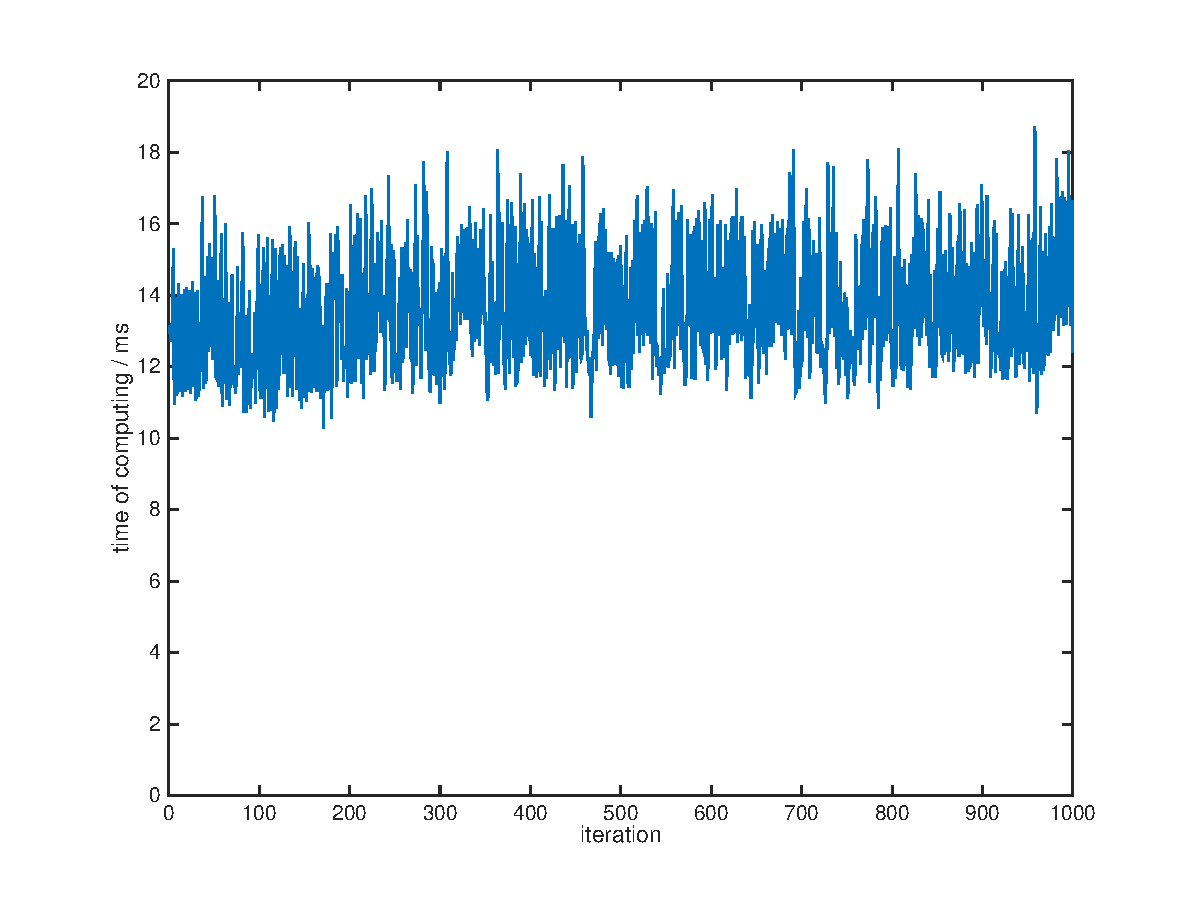
\includegraphics[width=12cm]{time_pthread}
    \fcaption{Time cost per each iteration (pthread)}\label{time_p}
\end{center}

\begin{center}
    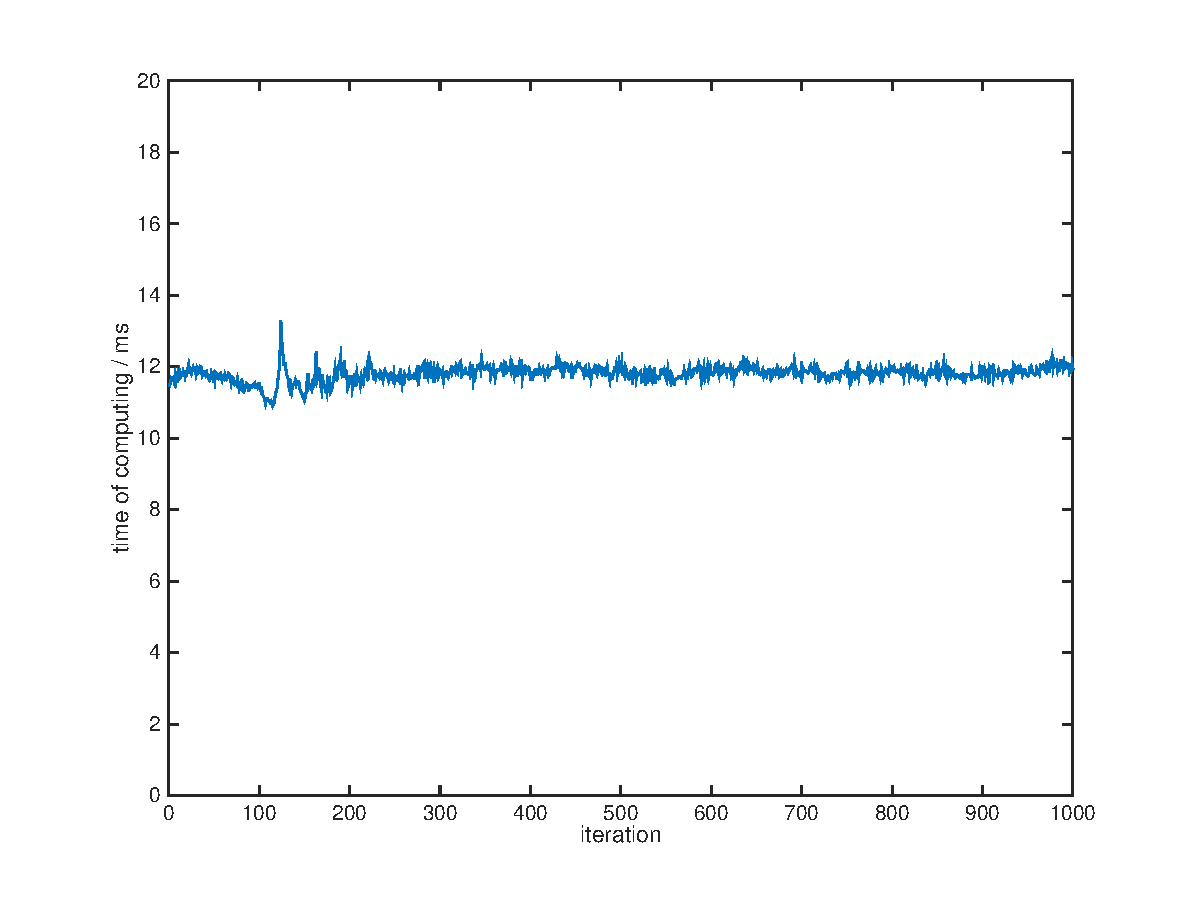
\includegraphics[width=12cm]{time_cuda}
    \fcaption{Time cost per each iteration (cuda)}\label{time_c}
\end{center}

We see that the time cost for each iteration is stable around 10ms. Thus, our ``reboucing strategy'' works.

\subsection{Number of Threads}

We use \texttt{test2.txt} as test case and we compute 10 iterations with mass 1, time interval 0.5 and threshold 1. The result is shown in \tref{p:not} and \fref{pf:not}. 

\begin{center}
    \tcaption{Performance on different number of threads}\label{p:not}
    \begin{tabular}{cc}
        \toprule
        number of threads & time of computing \\
        \midrule
        1 & 538.2566 \\ 
        2 & 292.9993 \\ 
        4 & 190.3291 \\ 
        8 & 104.7604 \\ 
        16 & 68.2259 \\ 
        32 & 62.0612 \\ 
        64 & 57.2310 \\ 
        128 & 53.4959 \\ 
        256 & 60.6209 \\ 
        \bottomrule
    \end{tabular}
\end{center}

\begin{center}
    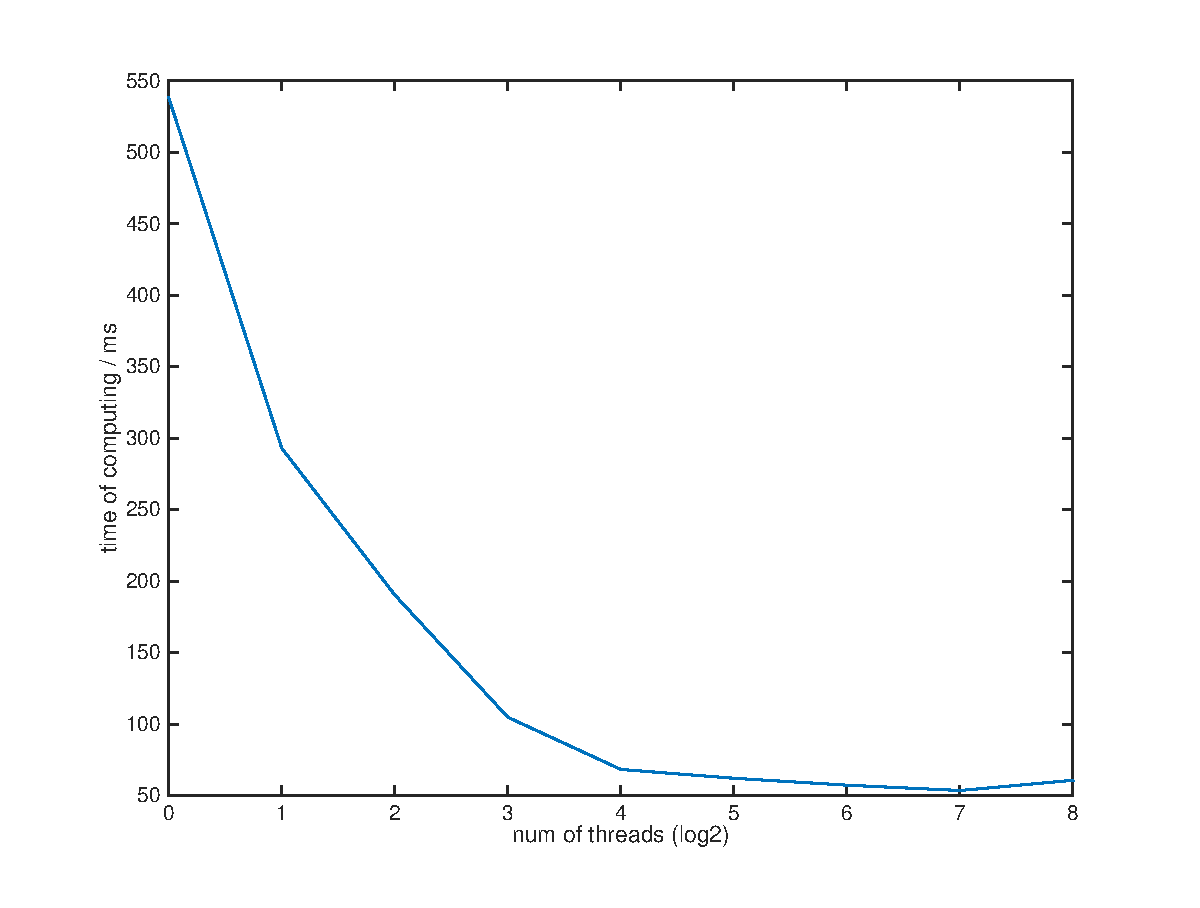
\includegraphics[width=12cm]{not}
    \fcaption{Performance on different number of threads}\label{pf:not}
\end{center}

We see that when the number of threads is doubled, the time of computing is not always halved. It is because we have a limit of threads that can run at the same time on a machine. Besides, more threads requires more time to create and more memory space to store data. If you create too many threads, the performance will not be good as expected.

\subsection{Threshold Value}

We use \texttt{test4.txt} as test case and we compute 10 iterations with mass 1 and time interval 0.001. Here we only use the cuda version. We see the relationship between performance and threshold in \fref{p:th}.

\begin{center}
    \tcaption{Performance on different threshold value}\label{p:th}
    \begin{tabular}{cc}
        \toprule
        threshold & time of computing \\
        \midrule
        0.5 & 14306.3809 \\
        1.0 & 3526.8691 \\
        1.5 & 1046.5911 \\
        2.0 & 222.5127 \\
    \bottomrule
    \end{tabular}
\end{center}

When we increase the threshold, we reduce the time of computing. In reality, the threshold parameter gives us a simple way to keep the trade-off between precision and performance. Large threshold leads to high performance but low precision, while small threshold leads to low performance but high precision. Large threshold can highly reduce the total depth of searching the quad-tree and thus saves a lot of time.

\subsection{Sample Size}

We first generate random samples in different size, i.e., $10^2, 10^3, \ldots, 10^7$ bodies respectively. The initial position is within range $(-1,1)$. The initial velocity is within range $(-0.1, 0.1)$.

Then we use these samples to test sequential version, pthread version and cuda version. We compute 10 iterations with mass 1, time interval 0.5 and threshold 1. The time cost and speed up is shown as \tref{p:sample}, where we define \textit{speed up} as
$$\mbox{speed up} = \frac{\mbox{sequential time}}{\mbox{cuda time}}$$
here. We see that by using 12 threads, the cuda version is faster than the pthread version when sample size is large. Also, speed up will be higher for larger sample.

\begin{center}
    \tcaption{Performance on different sample size}\label{p:sample}
    \begin{tabular}{ccccc}
        \toprule
        sample size & pthread time & cuda time & sequential time & speed up \\
        \midrule
        $10^2$ & 1.0750 & 0.9339 & 0.1046 & 0.1 \\ 
        $10^3$ & 1.2820 & 1.9371 & 1.7768 & 0.9 \\ 
        $10^4$ & 10.7835 & 4.2224 & 24.9308 & 5.9 \\ 
        $10^5$ & 87.6806 & 55.2118 & 250.8340 & 4.5 \\
        $10^6$ & 1731.9879 & 1165.7869 & 3841.7661 & 3.3 \\
        $10^7$ & 10264.4414 & 7107.6475 & 49441.0547 & 7.0 \\
        \bottomrule
    \end{tabular}
\end{center}

\section{Performance Results for Test Cases}

We now use the four given test cases to measure the performance of sequential version, pthread version and cuda version. We use 12 threads and mass 1 on all test cases and the results are shown in \tref{cases}.

\begin{center}
    \tcaption{Performance results for the given test cases}\label{cases}
    \begin{tabular}{ccccccccccc}
        \toprule
        test case & iteration & time interval & threshold & sequential & pthread & cuda \\
        \midrule
        \texttt{test1.txt} & 1000 & 0.5 & 0 & 72.5762 & 10.9493 & 11.8188 \\
        \texttt{test2.txt} & 100 & 0.01 & 1 & 490.3596 & 82.4046 & 34.6829 \\
        \texttt{test3.txt} & 10 & 0.01 & 1 & 22757.1484 & 2237.4797 & 1367.4998 \\
        \texttt{test4.txt} & 10 & 0.001 & 1 & 65673.0859 & 6030.9814 & 3524.6965 \\
        \bottomrule
    \end{tabular}
\end{center}

The speed up is shown in \tref{su} and \fref{su_fig}.

\begin{center}
    \tcaption{Speed up for the test cases}\label{su}
    \begin{tabular}{ccccccccccc}
        \toprule
        test case & speed up (pthread) & speed up (cuda) \\
        \midrule
        \texttt{test1.txt} & 6.6 & 6.1 \\
        \texttt{test2.txt} & 6.0 & 14.1 \\
        \texttt{test3.txt} & 10.2 & 16.6 \\
        \texttt{test4.txt} & 10.9 & 18.6 \\
        \bottomrule
    \end{tabular}
\end{center}

\begin{center}
    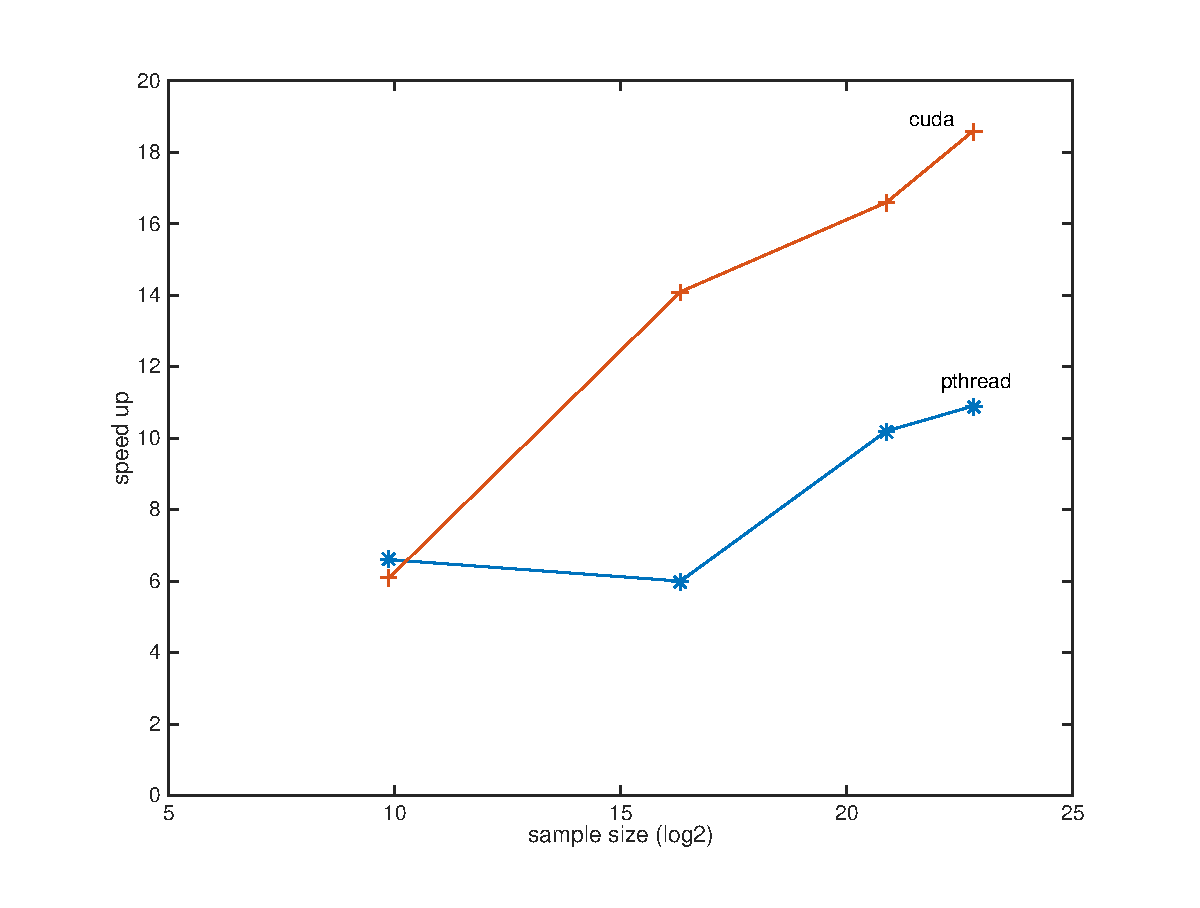
\includegraphics[width=12cm]{su}
    \fcaption{Speed up for the test cases}\label{su_fig}
\end{center}

\section{Further Discussion: Possible Improvements}

The following possible improvements can make higher performance:

\begin{itemize}
    \item dynamic task allocation for pthread,
    \item parallel tree constructing by area dividing,
    \item using non-recursive tree constructing method,
    \item using faster memory on GPU, for instance, shared memory for tree data,
    \item using faster square root computation algorithm on CPU, or compute square root using the hardware implementation on GPU (if avaiable),
    \item minimize the struct size of tree node for both smaller memory usage and faster memory access.
\end{itemize}

\section{Usage}

\subsection{Compiling}

In command line, type

\texttt{\$ make}

\subsection{Running}

\texttt{Usage: ./nbody num\_of\_threads m T t file $\theta$ enable/disable xmin ymin length Length}

The parameters mean:

\begin{itemize}
    \item \texttt{num\_of\_threads} number of threads to use for pthread version
    \item \texttt{m} mass for each body (float)
    \item \texttt{T} number of total iterations
    \item \texttt{t} time interval for each iteration (float)
    \item \texttt{file} input sample file (first line an integer $n$ showing the sample size, then the following $n$ lines shows the initial position $(x, y)$ and velocity $(v_x, v_y)$ for each body
    \item \texttt{$\theta$} threshold value (float)
    \item \texttt{enable/disable} enable/disable xwindow display
    \item \texttt{xmin, ymin} the lower left coordinate that xwindow displays (float)
    \item \texttt{length} the actual length of the coordinate axis stands for (float)
    \item \texttt{Length} xwindow's side length
\end{itemize}

\fref{ss1} and \fref{ss2} are screen shots.

\begin{center}
    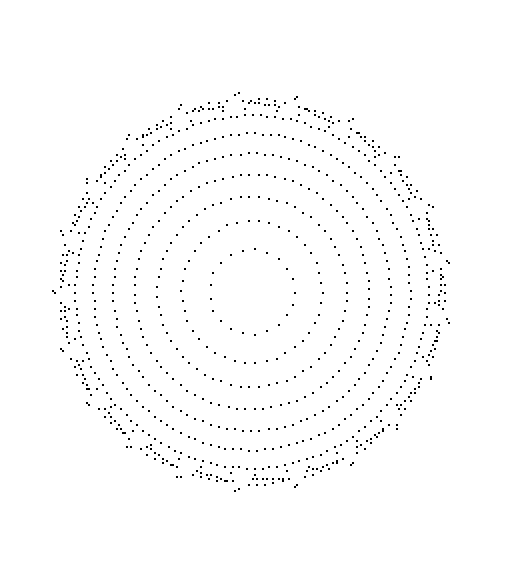
\includegraphics[width=10cm]{ss1}
    \fcaption{Screen shot for test1}\label{ss1}
\end{center}

\begin{center}
    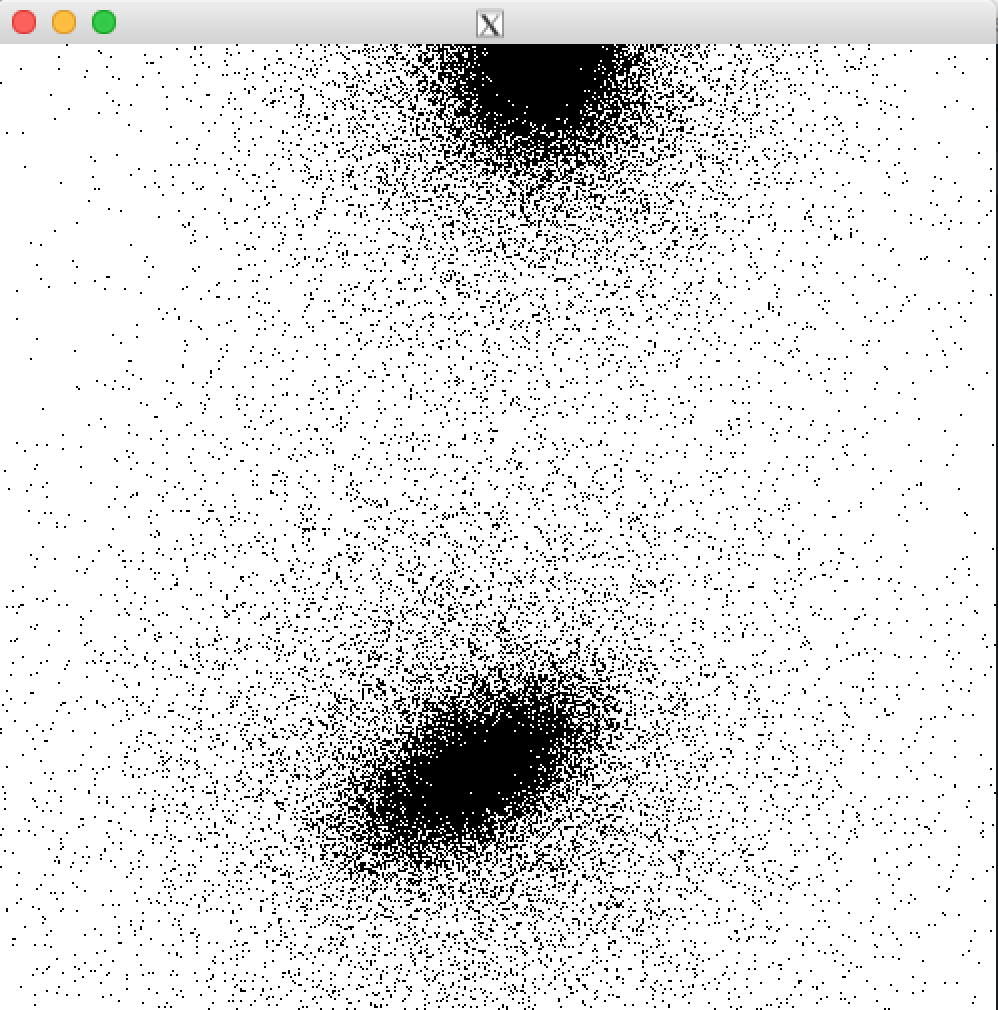
\includegraphics[width=10cm]{ss2}
    \fcaption{Screen shot for test2}\label{ss2}
\end{center}

\end{document}
